\paragraph{$K$-Means Clustering}
It is a method for finding clusters and cluster centers in a set of unlabeled data. 
\subparagraph{Definition}
The principle lays on the thought that a good clustering is one for
which the within cluster variation is as small as possible. The
within-cluster variation for cluster $C_{k}$is a measure $W(C_{k})$:
\begin{center}
\enc{
$
\min\limits_{\prth{C}{i}{K}}\left\{ \su{{k=1}}{K}W(C_{k}) \right\}
$
}
\end{center}
We need to define the within-cluster variation, the most common choice
is:
\begin{center}
\enc{
$
W(C_{k})=\dfrac{1}{|C_{k}|}\su{ {i,i'\in C_{k}}}{}\su{{j=1}}{p}(x_{ij}-x_{i'j})^{2}
$
}
\end{center}
where \tB{$|C_{k}|$ denotes the cardinal of $k^{th}$ cluster}.

\subparagraph{Algorithm K-Means Clustering}

\begin{enumerate}
	\item Randomly assign a number in $\inter{1}{K}$ to each of the
		observations.
	\item Iterate until the cluster assignment stop changing:
		\begin{enumerate}[label=(\alph*)]
			\item For each $K$ clusters, compute the
				cluster \emph{centroid}. The $k^{th}$
				cluster centroid is the vector of 
				the $p$ feature means for the 
				observations in the $k^{th}$ cluster.
			\item Assign each observation to the cluster
				whose centroid is closet.
			\end{enumerate}
\end{enumerate}
\begin{figure}[H]
	\begin{center}
		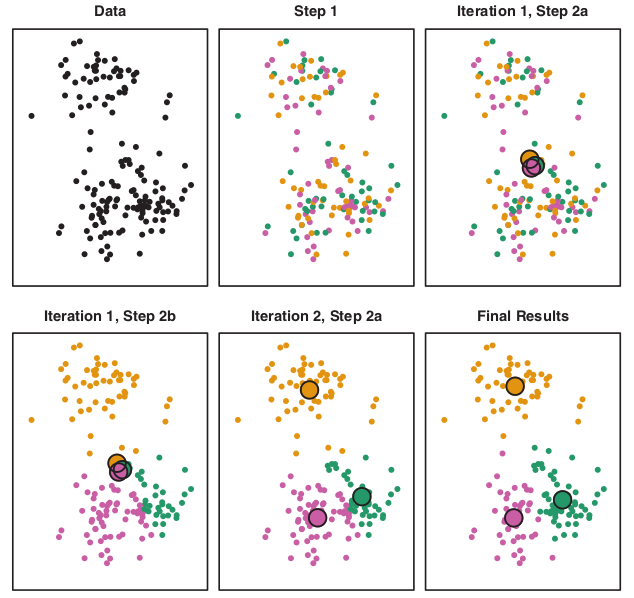
\includegraphics[width=.5\textwidth]{./chap/1chap/9sec/images/1kMeans.png}
	\end{center}
	\caption{Step1: Each observation is randomly assigned\\
	Step(2a): The clusters are computed\\
	Step(2b): Each observation is assigned to the nearest centroid.}
	\label{fig:9.1kMeans}
\end{figure}
\subparagraph{Python Code}
\begin{python}
import pandas as pd
import sklearn
from sklearn.cluster import KMeans

X = df.copy()
kmeans = KMeans(n_clusters=2,
    random_state=0).fit(X)
print(kmeans.labels_)
print(kmeans.cluster_centers_)
\end{python}

\subparagraph{Learning Vector Quantization}
In this technique, prototypes are placed strategically with respect to the decision boundaries
in an ad-hoc way. LVQ is an online algorithm. The idea is that the training points attract
prototypes of the correct class and repel other prototypes.
\begin{enumerate}
	\item Choose $R$ initial prototypes for each class: $\left\{m_{r}(k)|(r,k)\in\inter{1}{R}
		\times\inter{1}{K}\right\}$ by sampling $R$ training points at random from each
		class.
	\item Sample a training point $x_{i}$ randomly (with replacement):
		\begin{enumerate}[label=\alph*]
			\item if $g_{i}=k$ (i.e. they are in the same class), move the prototype
				towards the training point:
				$$ m_{j}(k)\leftarrow m_{j}(k) + \epsilon(x_{i}-m_{j}(k))$$
				where $\epsilon$ is the learning rate
			\item If $g_{i}\neq k$ (i.e, they are in different classes), move the 
				prototype away from the training point:
				$$ m_{j}(k)\leftarrow m_{j}(k) - \epsilon(x_{i}-m_{j}(k))$$
		\end{enumerate}
	\item Repeat step 2, decreasing the learning rate $\epsilon$ with each iteration towards
		zero.
\end{enumerate}

\paragraph{Hierarchical Clustering}
It is an alternative approach which does not require the we commit to
a particular choice of $K$.\\
It results in an attractive tree-based representation of the 
observations, called a \emph{dendrogram}.

\subparagraph{Interpreting a Dendogram}

\begin{figure}[H]
\begin{subfigure}[b]{0.49\textwidth}
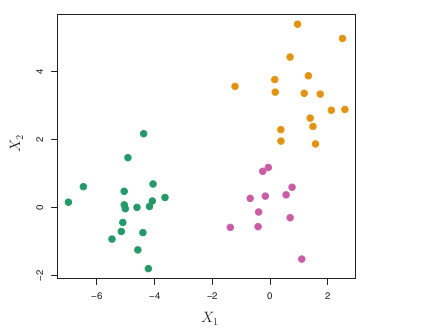
\includegraphics[width=\textwidth]{./chap/1chap/9sec/images/2a_hierarchicalCluster.png}
\caption{Original Data Set}
\label{fig:9.2a_hierarchicalCluster}
\end{subfigure}
\hfill
\begin{subfigure}[b]{0.49\textwidth}
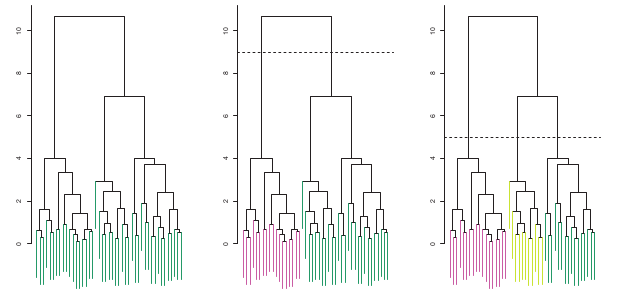
\includegraphics[width=\textwidth]{./chap/1chap/9sec/images/2b_hierarchicalCluster.png}
\caption{Dendrogram}
\label{fig:9.2b_hierarchicalCluster}
\end{subfigure}
\caption{
There are in reality 3 classes, but we will ignore them
and seek to cluster the observations.\\
In the right figure:\\
Left: Dendogram obtained from hierarchically clustering the data of of the left figure.\\
Center: The Dendrogram from the left-hand panel cut at a heigh of 9.
This cut results in 2 distinct clusters.\\
Right: The Dendrogram from the left-hand panel cut at a heigh of 5.
This cut results in 3 distincts clusters.
.}
\end{figure}

\subparagraph{Hierarchical Clustering}
\begin{enumerate}
	\item Begin with $n$ observations and a measure (such as 
		Euclidean distance) of all the $\binom{n}{2}$ pairwise
		dissimilarities.\\ \sB{Treat each observations as its own
		cluster}:
	\item $\forall i\in\inter{2}{n}$:
		\begin{enumerate}
			\item Examine all pairwise inter-cluster 
				dissimilarities among the $i$ cluster
				and \sB{identify the pair of clusters that
				are least dissimilar.\\
				Fuse these 2 cluster}, the dissimilarity
				between these 2 clusters indicates
				the height of the dendrogram at which
				the fusion should be placed.
			\item \sB{Compute the new pairwise inter-cluster
				dissimilarities among the $i-1$
				remaining clusters.}

		\end{enumerate}
\end{enumerate}

\subparagraph{Python Code}
\begin{python}
import pandas as pd
import sklearn
from sklearn.cluster import AgglomerativeClustering

X = df.copy()
clustering = AgglomerativeClustering().fit(X)
print(clustering.labels_)
\end{python}
\paragraph{Adaptive Nearest-Neighbor Methods}
When nearest-neighbor classification is carried out in a high-dimensional feature space, the
nearest neighbors of a point can be very far away, causing bias.\\
To quantify this, consider $N$ data points uniformly distributed in the unit cube $\left[-\dfrac{
1}{2},\dfrac{1}{2}\right]^{p}$. Let $R$ be the radius of a 1-nearest-neighborhood centered at the
origin. Then:
$$ median(R)=v_{p}^{-\frac{1}{p}}\left(1-\dfrac{1}{2}^{\frac{1}{N}}\right)^{\frac{1}{p}}$$ where
$v_{p}r^{^p}$ is the volume of the sphere of radius $r$ in $p$ dimensions.\\

The \emph{Discriminant Adaptive Nearest-Neighbor} (DANN) metric at a query point $x_{0}$ is 
defined by : 
$$ D(x, x_{0}) = (x-x_{0})^{T}\bm{\Sigma}(x-x_{0})$$ where 
\begin{align*}
	\bm{\Sigma} =& \bm{W}^{-\frac{1}{2}}\left[\bm{W}^{-\frac{1}{2}}\bm{B}\bm{W}^{-\frac{1}{2}}
	+\epsilon \bm{I}\right]\bm{W}^{-\frac{1}{2}}\\
	=& \bm{W}^{-\frac{1}{2}}\left[\bm{B}^{*}+\epsilon\bm{I}\right]\bm{W}^{-\frac{1}{2}}
\end{align*}

Here $\bm{W}$ is the pooled within-class covariance matrix $\su{{k=1}}{K}\pi_{k}\bm{W}_{k}$ and
$\bm{W}$ is the between class covariance matrix $\su{{k=1}}{K}\pi_{k}\left(\overline{x}_{k}-
\overline{x}\right)\left(\overline{x}_{k}-\overline{x}\right)$ with $\bm{W}$ and $\bm{B}$
computed using only the $50$ nearest neighbors around $x_{0}$.
